\chapter{Orçamento do Steve}
\label{ch:identificador}

\section{Custos de implementação}
Inicialmente realizaremos a implementação do Steve Robot Express nas principais capitais e regiões metropolitanas das regiões Sul, Sudeste e Centro Oeste totalizando onze capitais para comercialização, realizando em média dez implementações mensais em cada uma das capitais totalizando 110 implementações ao mês 1.320 por ano.

\section{Custo do robô Steve}
Nossos robôs Steve são produzidos em parceria com a empresa Synkar,
companhia brasileira especializada em inteligência artificial que disponibiliza toda a parte de software, automação, manutenção e reposição de peças. O valor de produção robô Steve e entorno de US\$ 5.000 em reais R\$ 26.036,00 com base no valor dos robôs da empresa Starship Technologies.

\section{Custo médio do ponto de recarga}
O valor gasto na adequação dos condomínios ficaria algo entre US\$ 288,06 a US\$ 960,21 dólares em reais algo entre R\$1.500,00 a R\$5.000.00 totalizando um custo médio de US\$ 624,14 dólares R\$ 3.250,00 reais. Pois para a implementação dos pontos de recarga são necessários um projeto elétrico que contenha desenho da rede elétrica cálculos de dimensões e especificações dos equipamentos utilizados também e necessário a ART (Anotação de Responsabilidade Técnica) que é um documento padrão de engenharia registrado junto ao CREA da documentação técnica do projeto. Os valores acima foram baseados em carregadores de automóveis elétricos de um artigo do site CondoCash \cite{CondoCash}.

\section{Instalação hardware e software IoT para elevador}
Para instalação dos sistemas de hardware e software realizamos uma parceria com uma grande empresa chinesa Dusun IoT \cite{DusunIot} especializada em hardware gateways IoT permitindo a comunicação do Steve com o elevador além dessa comunicação permitirá que o condomínio tenha em mãos dados de monitoramento em tempo real e desempenho do elevador, possibilitando a manutenção preditiva prevendo falhas antes que ocorram e otimização do consumo de energia do elevador com base em dados pesquisados os custos de hardware com sensores, módulos Wi-Fi, Bluetooth, Placas como o Raspberry Pi, Arduino, câmeras de segurança IoT, rastreadores GPS, placas, cabos e documentação variando de R\$ 1.500,00 a R\$ 1.800,00 reais, com um custo médio de R\$ 1.650,00 reais. Os valores das peças foram retirados dos principais Marketplaces do Brasil. Já o software ficara em torno de US\$ 10.000,00 dólares algo entre R\$52.072 reais em valores aproximados de acordo com o site ICHI.PRO \cite{ICHI.PRO} mas uma vez desenvolvido o software poderia ser usado utilizado em todas as instalações havendo apenas pequenas atualizações. 

\section{Custos operacionais mensais nas onze capitais}
Os custos operacionais relacionados a reposição de peças em estoque totalizam R\$ 2.000,00 reais por capital totalizando um custo mensal nas onze capitais de R\$ 22.000,00, além do custo das peças temos os custos com técnico de mecatrônica que é de R\$ 5.200,00 reais por capital totalizando um custo mensal com técnicos de R\$ 57.200,00 reais nas onze capitais. Totalizando R\$ 79.400,00 de custos operacionais mensais.

\section{Custos totais para viabilização da Steve Robot Express}
Com um investimento inicial de R\$ 90.208,00 para a viabilização da Steve Robot Express, na primeira capital, mas vendo abaixo um modelo de implementação ficara mais claro ver que o retorno do investimento e muito atrativo e escalável trazendo retornos consideráveis em alguns anos.

\textbf{Exemplo de implantação}
Dados de implementação do Steve Robot Express em um condomínio com 328 residentes que necessitaria de dois Steve Robots para realização de todas as entregas.

\textbf{Dados usados para a base de cálculo:}
\begin{itemize}
    \item Custo Steve Robot 2 unidades: R\$ 52.072,00
    \item Custo Bases de recarga 1 unidade: R\$ 3.250,00
    \item Custo médio Elevador Smart hardware 2 unidades: R\$ 3.300,00
    \item custos operacionais mensais: R\$ 7.200,00
    \item custo total para implementação: R\$ 65.822,00
    \item Valor recebido do condomínio para implementação: R\$ 100.000,00
    \item Parcelas mensais recebidas do condomínio para 2 unidades do Steve Robot: R\$ 8.250,00
\end{itemize}

\textbf{Cálculo implantação:}
Para calcular o lucro retorno sobre o investimento em um período de doze meses, realizaremos a subtração dos custos totais do valor recebido durante o período de doze meses.

Custo Total= R\$ 65.822,00 + R\$ 86.400,00 = R\$ 152.222,00 reais, o custo total e a soma da implantação mais os custos operacionais durante os doze meses.

Agora calcularemos o valor recebido da implantação mais os pagamentos mensais.

Valor Total Recebido = R\$ 100.000,00 + R\$ 99.000,00 = R\$ 199.000,00 reais

Agora para calcular o retorno sobre o investimento, vamos subtrair o custo total do valor total recebido.

Lucro / Retorno = R\$ 199.000,00 – R\$ 152.222,00 = R\$ 46.778,00 reais

Após os cálculos concluímos que o retorno sobre o investimento para a implementação do Steve Robot Express retornaria ao final de doze meses 30,75\% totalizando um lucro de R\$ 46.778,00 da implementação em apenas um condomínio. 

\section{Retorno dos investimentos da Steve Robot Express}
Com o lucro de apenas uma implementação retornando R\$ 46.778,00 reais se multiplicarmos esse valor por 110 implementações mensais teríamos o valor de R\$ 5.145.580,00 reais que em um ano seria o equivalente a R\$ 61.746.960,00.

Estudo da consultoria Boston Consulting Group (BCG) \cite{(BCG)} prevê que robôs de serviço deverão se tornar líderes no setor da robótica até o final da década o que representaria US\$ 90 bilhões a US\$ 170 bilhões do faturamento global em 2030 para a categoria. O estudo abrange diversas mudanças elas estão relacionadas ao envelhecimento da população que necessitarão de ajuda na realização de tarefas, mudanças no comportamento da população aumentando a demanda de entregas de produtos cada vez mais rápida e personalizada sem falar da conscientização da população em relação a ações mais sustentáveis que levarão a modernização e maior uso dos robôs.

Outra previsão realizada prevê que o tamanho mercado de robótica é estimado em US\$ 45,85 bilhões em 2024, e deverá atingir US\$ 95,93 bilhões até 2029, crescendo a um CAGR de 15,91\% durante o período de previsão (2024-2029). Foi observado numerosos investimentos no setor por conta da revolução da Industria 4.0 que são um dos elementos chave para o desenvolvimento dos robôs o gráfico abaixo mostra uma projeção do desenvolvimento e crescimento do mercado até onfim dessa década. 

\begin{figure} [!ht]
    \centering
    \caption{Indústria de robótica - Análise de tamanho e participação - Tendências e previsões de crescimento (2024 - 2029)}
    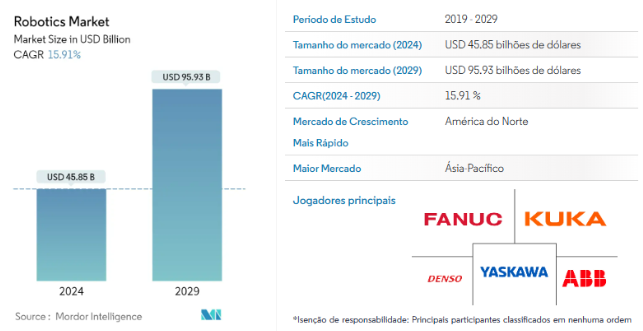
\includegraphics[width=0.9\linewidth]{figuras/orça drop.png}
    \label{fig:enter-label}
    \fonte{Mordor Intelligence Research & Advisory}
\end{figure}

Com as previsões dessas instituições fica claro que o cenário da robótica só está no começo como uma empresa pioneira a Drop Flash vem com missão de a cada dia aproximar o cidadão comum com tecnologias que em alguns anos se tornarão essenciais para garantir a qualidade nas entregas. 